% !TeX spellcheck = es_CL-SpanishChile
\documentclass[aspectratio=1610]{beamer}

\usepackage{tikz}
\usepackage{./SimonPackage}
\newcommand{\Ev}{\Vec{E}}
\newcommand{\kv}{\Vec{\kappa}}

\definecolor{myaccent}{HTML}{356AE6}
\usetheme[
accent=myaccent,
progressbar=foot,
sectionpage=progressbar,
subsectionpage=progressbar,
numbering=fraction,
block=fill
]{cookie}

\title{Radiación de Cuerpo Negro, Física Estadística}
\author{Simón Fonseca}
\date{25 Junio, 2026}

\begin{document}
\maketitle

%%%%%%%%%%%%%%%%%%%%%%%%%%%%%%%%%%%%%%%%%%%%%%%%%%%%%%%%%%%%%%%%%%%%%%%%%%%%%%%%%%
\section{Estados cuánticos de una partícula}
\begin{frame}{Estadística fotónica}{}
	\begin{itemize}
		\item Consideremos radiación electromagnética, una colección de fotones indistinguibles, dentro de una caja de lados $L_x,L_y,L_z$.
		% Deben ser indistinguibles, obviamente
		\item La cantidad total de fotones no es fija, depende de la temperatura $T$ de las paredes.\pause
		\item El campo de radiación en equilibrio térmico dentro de una caja está completamente descrito la distribución de Planck, que se expresa como:
		\begin{equation}
			\bar{n}_s = \frac{1}{e^{\beta \epsilon_s}-1},
			\label{eq:planck}
		\end{equation}
		donde $\bar{n}_s$ es el número promedio de fotones en el estado $s$, y $\epsilon_s$ es la energía asociada a tal estado.
	\end{itemize}
\end{frame}

\begin{frame}
	\begin{itemize}
		\item Debido a la naturaleza periódica de la ecuación de onda espacial de los fotones $\vec{\psi}(\vec{r})=e^{i\kv\cdot\vec{r}}$, se requiere que
		\begin{equation}
			\kappa_i=\frac{2\pi}{L_i}n_i ,
		\end{equation}
		donde $i$ es cualquier dirección del espacio, y $n_i$ es un número entero.\pause
		\item Luego, el número $\Delta n_i$ de posibles enteros $n_i$ para los cuales $\kappa_i$ está dentro del rango $\kappa_i$ y $\kappa_i+d\kappa_i$ es igual a
		\begin{equation}
			\Delta n_i=\frac{L_i}{2\pi}d\kappa_i
		\end{equation}\pause
		\item Por lo que, finalmente, el número de estados $\rho(\kv)d^3\kv$, para los cuales $\kv$ se encuentra dentro del rango $\kv$ y $\kv+d\kv$, estará dado por
	\end{itemize}
	
	\begin{equation}
		\rho \, d^3\kv = \Delta n_x \Delta n_y \Delta n_z = \left(\frac{L_x}{2\pi}d\kappa_x \right) \left(\frac{L_y}{2\pi}d\kappa_y \right) \left(\frac{L_y}{2\pi}d\kappa_y \right) = \frac{V}{(2\pi)^3}d^3\kv
		\label{eq:NumEstados}
	\end{equation}
\end{frame}
	
%%%%%%%%%%%%%%%%%%%%%%%%%%%%%%%%%%%%%%%%%%%%%%%%%%%%%%%%%%%%%%%%%%%%%%%%%%%%%%%%%%
\section{Radiación en equilibrio térmico}
\begin{frame}{Radiación en equilibrio}
	\begin{itemize}
		\item Para especificar con más detalle los estados de energía, consideraremos la ecuación de onda del campo eléctrico $\Ev$
		\begin{equation}
			\nabla^2\Ev=\frac{1}{c^2}\frac{\partial \Ev}{\partial t}
			\label{eq:EWave}
		\end{equation}\pause
		\item La cual es satisfecha por
		\begin{equation}
			\Ev = \Vec{A} e^{i (\kv\cdot\Vec{r}-\omega t)} = \Ev_0 e^{-i \omega t},
			\label{eq:ESol}
		\end{equation}
		donde $\Vec{A}$ es cualquier constante, y $\kv$ cumple con la condición
		\begin{equation}
			\kappa = \frac{\omega}{c}, \qquad \kappa = |\kv|
			\label{eq:kappa}
		\end{equation}
	\end{itemize}
\end{frame}

\begin{frame}
	\begin{itemize}
		\item Si ahora cuantizamos la ecuación de onda, llegaremos a las típicas relaciones de momento y energía para un fotón asociado:
		\begin{equation}
			\begin{array}{rcl}
				\epsilon &=& \hbar \omega  \\
				\Vec{p} &=& \hbar \kv 
			\end{array},
			\label{eq:EMom}
		\end{equation}
		por lo que, con la ec. \ref{eq:kappa}
		\begin{equation}
			|\Vec{p}| = \frac{\hbar \omega}{c}
		\end{equation}\pause
		\item Ya que $\kv$ debe ser perpendicular a $\Ev$, tendremos dos polarizaciones disponibles para el campo eléctrico.
	\end{itemize}
\end{frame}

\begin{frame}
	\begin{itemize}
		\item Como cualquier partícula cuántica dentro de una caja, solo hay ciertos valores válidos para $\kv$, dependientes de las dimensiones de la caja $L_x,L_y,L_z$.\pause
		\item Suponemos que la más pequeña de estas dimensiones, $L$, es tan larga para $L \gg \lambda$, donde $\lambda = \frac{2\pi}{\kappa}$ es la mayor longitud de onda en discusión.\pause
		% Con esto nos evitamos efectos que puedan ocurrir cerca de las paredes de la caja
		\item Los valores posibles de $\kv$ estarán dados por los de
	\end{itemize}\pause
	\begin{block}{Densidad promedio de fotones}
		$f(\kv)d^3\kv =$ el número promedio de fotones por unidad de volumen, que tienen una dirección específica de polarización, y cuyos vectores de onda existen entre $\kv$ y $\kv+d\kv$.
	\end{block}
\end{frame}

\begin{frame}
	\begin{itemize}
		\item Hay, según la ec. \ref{eq:NumEstados}, $(2\pi)^{-3}d^3\kv$ estados para los fotones por unidad de volumen, y, ya que la cantidad de fotones en cada estado de energía vienen dado por la ec. \ref{eq:planck}, tenemos que
		\begin{equation}
			f(\kappa) \, d^3\kappa = \frac{1}{e^{\beta \hbar \omega}-1} \frac{d^3\kappa}{(2\pi)^3}
			\label{eq:DensFot}
		\end{equation}\pause
		\item Encontremos ahora el número promedio de fotones por unidad de volumen en ambas direcciones de polarización y con frecuencia en el rango entre $\omega$ y $\omega+d\omega$.\pause
		\item Podemos encontrarlo si integramos la ec. \ref{eq:DensFot} sobre el volumen del espacio $\kappa$ contenido dentro de una capa esférico de radios $\kappa = \omega/c$ y $\kappa+d\kappa = (\omega+d\omega)/c$. % Y multiplicando por 2 por ambas polarizaciones
		\begin{equation}
			2 f(\kappa) \, (4\pi\kappa^2d\kappa) = \dfrac{8\pi}{(2\pi c)^3}\dfrac{\omega^2d\omega}{e^{\beta\hbar\omega}-1}
		\end{equation}
	\end{itemize}
\end{frame}

\begin{frame}
	\begin{itemize}
		\item Denotando con $\bar{u}(\omega,T) \, d\omega$ la energía media por unidad de volumen (es decir, la \emph{densidad de energía} promedio) de fotones en ambas direcciones de polarización en el rango de frecuencias $\omega$ y $\omega+d\omega$.\pause
		\item Ya que cada fotón de este tipo tiene una energía $\hbar\omega$, se obtiene
		\begin{equation}
			\bar{u}(\omega,T)d\omega = (2 f(\kappa)\hspace{1mm}4\pi\kappa^2d\kappa)\hspace{1mm}(\hbar\omega) = \dfrac{8\pi\hbar}{c^3}f(\kappa)\hspace{1mm}\omega^3d\omega
			\label{eq:DensEnerProm}
		\end{equation}
	\end{itemize}
\end{frame}

%%%%%%%%%%%%%%%%%%%%%%%%%%%%%%%%%%%%%%%%%%%%%%%%%%%%%%%%
\section{Radiación emitida a temperatura $T$}
\begin{frame}{Radiación emitida por un cuerpo a temperatura $T$}
	\begin{itemize}
		\item Consideremos un cuerpo mantenido a una temperatura absoluta $T$, por ejemplo, el filamento caliente de una ampolleta.\pause
		\item Sabemos que este cuerpo emite radiación electromagnética.\pause
		\item Y estamos interesados en cuanta energía por unidad de tiempo (potencia) $P(\omega)d\omega$ que emite este cuerpo en el rango de frecuencia  entre $\omega$ y $\omega+d\omega$.
	\end{itemize}
\end{frame}

\begin{frame}{Cuerpos como emisores y receptores de radiación}
	\begin{itemize}
		\item Consideremos un cuerpo arbitrario a temperatura absoluta $T$.\pause
		\item La radiación emitida por este cuerpo puede ser descrita en términos de su potencia.\pause
		\item Podemos definir la \emph{emisividad} como\pause
		\begin{block}{Emisividad}
			$\mathcal{P}_e(\kv,\alpha)d\omega d\Omega = $ la potencia, por unidad de área, emitida con polarización $\alpha$ y en el rango alrededor de $\kv$ (es decir, en el rango de frecuencia $\omega + d\omega$, y con un ángulo sólido $d\Omega$ en torno a $\kv$).
		\end{block}\pause
		\item La emisividad depende de la naturaleza del material y de su temperatura.
	\end{itemize}
\end{frame}

\begin{frame}
	\begin{itemize}
		\item Ahora para un receptor de radiación, consideraremos radiación de polarización $\alpha$ en el rango alrededor $\kv'$.\pause
		\item Supongamos que la radiación de este tipo es \emph{incidente}, tal que la potencia $\mathcal{P}_i(\kv';\alpha)d\omega d\Omega$ es incidente por unidad de área del cuerpo.\pause
		\item De esto, solo una fracción $a(\kv,\alpha)$, llamada \emph{absorvencia}, es absorbida por el cuerpo.\pause
		\item $a(\kv,\alpha)$ es característica de un cuerpo y depende, en general, de la temperatura $T$.\pause
	\end{itemize}
	\begin{figure}
		\centering
		
		
		\tikzset{every picture/.style={line width=0.75pt}} %set default line width to 0.75pt        
		
		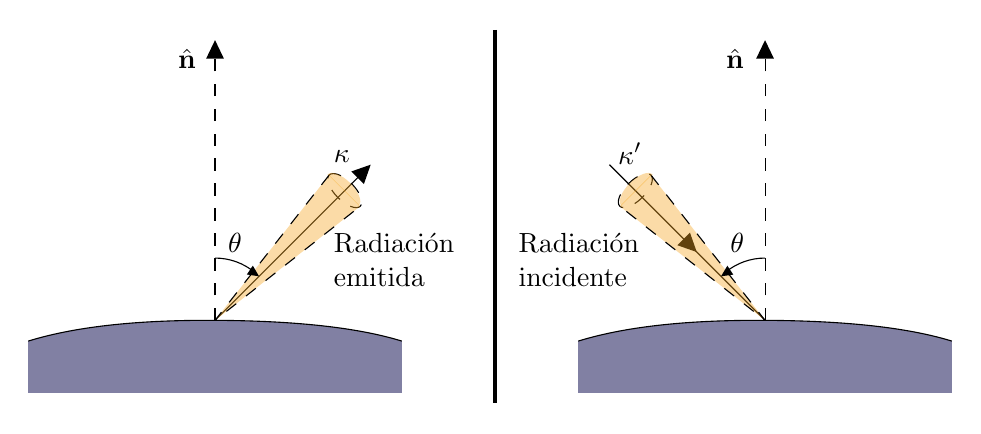
\begin{tikzpicture}[x=0.75pt,y=0.75pt,yscale=-1,xscale=1]
			%uncomment if require: \path (0,300); %set diagram left start at 0, and has height of 300
			
			%Straight Lines [id:da6678405234062144] 
			\draw  [dash pattern={on 4.5pt off 4.5pt}]  (150,160) -- (150,28) ;
			\draw [shift={(150,25)}, rotate = 90] [fill={rgb, 255:red, 0; green, 0; blue, 0 }  ][line width=0.08]  [draw opacity=0] (8.93,-4.29) -- (0,0) -- (8.93,4.29) -- cycle    ;
			%Straight Lines [id:da30725018613871535] 
			\draw    (150,160) -- (222.88,87.12) ;
			\draw [shift={(225,85)}, rotate = 135] [fill={rgb, 255:red, 0; green, 0; blue, 0 }  ][line width=0.08]  [draw opacity=0] (8.93,-4.29) -- (0,0) -- (8.93,4.29) -- cycle    ;
			%Shape: Ellipse [id:dp024683953439570194] 
			\draw  [dash pattern={on 4.5pt off 4.5pt}] (205,90) .. controls (206.83,88.17) and (211.68,90.04) .. (215.82,94.18) .. controls (219.96,98.32) and (221.83,103.17) .. (220,105) .. controls (218.17,106.83) and (213.32,104.96) .. (209.18,100.82) .. controls (205.04,96.68) and (203.17,91.83) .. (205,90) -- cycle ;
			%Straight Lines [id:da27781945716401235] 
			\draw [fill={rgb, 255:red, 245; green, 166; blue, 35 }  ,fill opacity=0.4 ] [dash pattern={on 4.5pt off 4.5pt}]  (205,90) -- (150.61,159.23) -- (150,160) -- (220,105) ;
			%Shape: Path Data [id:dp7177920702073797] 
			\draw  [draw opacity=0][fill={rgb, 255:red, 245; green, 166; blue, 35 }  ,fill opacity=0.4 ][dash pattern={on 4.5pt off 4.5pt}] (215.12,93.86) .. controls (219.26,98.01) and (221.13,102.85) .. (219.3,104.69) .. controls (219.17,104.81) and (219.04,104.91) .. (218.9,105) -- (219.3,104.69) -- (204.3,89.69) -- (203.98,90.09) .. controls (204.07,89.94) and (204.17,89.81) .. (204.3,89.69) .. controls (206.13,87.85) and (210.97,89.72) .. (215.12,93.86) -- cycle ;
			%Shape: Arc [id:dp10702653053025535] 
			\draw  [draw opacity=0] (150,130) .. controls (150,130) and (150,130) .. (150,130) .. controls (158.28,130) and (165.78,133.36) .. (171.21,138.79) -- (150,160) -- cycle ; \draw    (150,130) .. controls (150,130) and (150,130) .. (150,130) .. controls (157.21,130) and (163.82,132.54) .. (168.99,136.78) ; \draw [shift={(171.21,138.79)}, rotate = 214.04] [fill={rgb, 255:red, 0; green, 0; blue, 0 }  ][line width=0.08]  [draw opacity=0] (5.36,-2.57) -- (0,0) -- (5.36,2.57) -- cycle    ; 
			%Straight Lines [id:da549387921188401] 
			\draw [line width=1.5]    (285,20) -- (285,200) ;
			%Shape: Rectangle [id:dp589233359798815] 
			\draw  [draw opacity=0][fill={rgb, 255:red, 129; green, 128; blue, 163 }  ,fill opacity=1 ] (325,170) -- (505,170) -- (505,195) -- (325,195) -- cycle ;
			%Straight Lines [id:da1777224502907243] 
			\draw  [dash pattern={on 4.5pt off 4.5pt}]  (415,160) -- (415,28) ;
			\draw [shift={(415,25)}, rotate = 90] [fill={rgb, 255:red, 0; green, 0; blue, 0 }  ][line width=0.08]  [draw opacity=0] (8.93,-4.29) -- (0,0) -- (8.93,4.29) -- cycle    ;
			%Straight Lines [id:da025460235534299214] 
			\draw    (415,160) -- (340,85) ;
			\draw [shift={(382.1,127.1)}, rotate = 225] [fill={rgb, 255:red, 0; green, 0; blue, 0 }  ][line width=0.08]  [draw opacity=0] (8.93,-4.29) -- (0,0) -- (8.93,4.29) -- cycle    ;
			%Shape: Ellipse [id:dp04887392986368977] 
			\draw  [dash pattern={on 4.5pt off 4.5pt}] (345,105) .. controls (343.17,103.17) and (345.04,98.32) .. (349.18,94.18) .. controls (353.32,90.04) and (358.17,88.17) .. (360,90) .. controls (361.83,91.83) and (359.96,96.68) .. (355.82,100.82) .. controls (351.68,104.96) and (346.83,106.83) .. (345,105) -- cycle ;
			%Straight Lines [id:da20083061057194007] 
			\draw [fill={rgb, 255:red, 245; green, 166; blue, 35 }  ,fill opacity=0.4 ] [dash pattern={on 4.5pt off 4.5pt}]  (360,90) -- (414.39,159.23) -- (415,160) -- (345,105) ;
			%Shape: Path Data [id:dp896698744356572] 
			\draw  [draw opacity=0][fill={rgb, 255:red, 245; green, 166; blue, 35 }  ,fill opacity=0.4 ][dash pattern={on 4.5pt off 4.5pt}] (349.88,93.86) .. controls (345.74,98.01) and (343.87,102.85) .. (345.7,104.69) .. controls (345.83,104.81) and (345.96,104.91) .. (346.1,105) -- (345.7,104.69) -- (360.7,89.69) -- (361.02,90.09) .. controls (360.93,89.94) and (360.83,89.81) .. (360.7,89.69) .. controls (358.87,87.85) and (354.03,89.72) .. (349.88,93.86) -- cycle ;
			%Shape: Arc [id:dp9530324867883474] 
			\draw  [draw opacity=0] (393.79,138.79) .. controls (399.22,133.36) and (406.72,130) .. (415,130) .. controls (415,130) and (415,130) .. (415,130) -- (415,160) -- cycle ; \draw    (396.1,136.7) .. controls (401.26,132.51) and (407.83,130) .. (415,130) ;  \draw [shift={(393.79,138.79)}, rotate = 326.62] [fill={rgb, 255:red, 0; green, 0; blue, 0 }  ][line width=0.08]  [draw opacity=0] (5.36,-2.57) -- (0,0) -- (5.36,2.57) -- cycle    ;
			%Shape: Rectangle [id:dp44786582319245827] 
			\draw  [draw opacity=0][fill={rgb, 255:red, 129; green, 128; blue, 163 }  ,fill opacity=1 ] (60,170) -- (240,170) -- (240,195) -- (60,195) -- cycle ;
			%Curve Lines [id:da18595315206886276] 
			\draw [fill={rgb, 255:red, 129; green, 128; blue, 163 }  ,fill opacity=1 ]   (325,170) .. controls (349.88,162.33) and (381.42,159.82) .. (415,160) .. controls (448.58,160.18) and (481.23,162.67) .. (505,170) ;
			%Curve Lines [id:da025409644954340282] 
			\draw [fill={rgb, 255:red, 129; green, 128; blue, 163 }  ,fill opacity=1 ]   (60,170) .. controls (84.88,162.33) and (116.42,159.82) .. (150,160) .. controls (183.58,160.18) and (216.23,162.67) .. (240,170) ;
			
			% Text Node
			\draw (131,28) node [anchor=north west][inner sep=0.75pt]   [align=left] {$\displaystyle \hat{\mathbf{n}}$};
			% Text Node
			\draw (155,117) node [anchor=north west][inner sep=0.75pt]   [align=left] {$\displaystyle \theta $};
			% Text Node
			\draw (206,77) node [anchor=north west][inner sep=0.75pt]   [align=left] {$\displaystyle \kappa $};
			% Text Node
			\draw (206,117) node [anchor=north west][inner sep=0.75pt]   [align=left] {Radiación\\emitida};
			% Text Node
			\draw (395,28) node [anchor=north west][inner sep=0.75pt]   [align=left] {$\displaystyle \hat{\mathbf{n}}$};
			% Text Node
			\draw (397,117) node [anchor=north west][inner sep=0.75pt]   [align=left] {$\displaystyle \theta $};
			% Text Node
			\draw (343,73) node [anchor=north west][inner sep=0.75pt]   [align=left] {$\displaystyle \kappa '$};
			% Text Node
			\draw (295,117) node [anchor=north west][inner sep=0.75pt]   [align=left] {Radiación\\incidente};
			
			
		\end{tikzpicture}
		
		
		\caption{Diagrama para la emisión y absorción de radiaciones por un cuerpo.}
		\label{fig:EmiAbs}
	\end{figure}
	%\citar{[1] Reif, F. (2009). \emph{Fundamentals of statistical and thermal physics}. Waveland Press.}
\end{frame}

\begin{frame}{El principio de equilibrio detallado}
	\begin{itemize}
		\item Imaginemos que el cuerpo estudiado se encuentra encerrado por una caja a la misma temperatura $T$, tal que esté en equilibrio con el campo de radiación interno.\pause
		\item Bajo estas condiciones, el cuerpo emite radiación. Por otro lado, también absorbe una cierta fracción de la radiación continuamente incidente.\pause
		\item Debido a la condición de equilibrio, la energía total del cuerpo debe ser constante; por lo tanto, los procesos deben balancearse tal que
		\begin{block}{}
			\centering
			Potencia radiada por el cuerpo = Potencia absorbida por el cuerpo
		\end{block}
	\end{itemize}
\end{frame}

\begin{frame}
	\begin{columns}
		\column{0.65\textwidth}
		\begin{itemize}
			\item Ahora, imaginemos que el cuerpo está rodeado por un filtro, que absorbe toda la radiación, a excepción de un pequeño elemento de área, donde es transparente para radiación de cierta polarización y un rango estrecho de frecuencia $\omega+d\omega$.\pause
			\item Debido a que la situación de equilibrio puede mantenerse sin importar la presencia del filtro, el balanceo de energía debe cumplirse para este elemento de área, polarización y frecuencia.\pause
			\item Como el filtro elegido era arbitrario, podemos concluir que
		\end{itemize}
		
		\column{0.35\textwidth}
		\begin{figure}
			\centering
			
			
			\tikzset{every picture/.style={line width=0.75pt}} %set default line width to 0.75pt        
			
			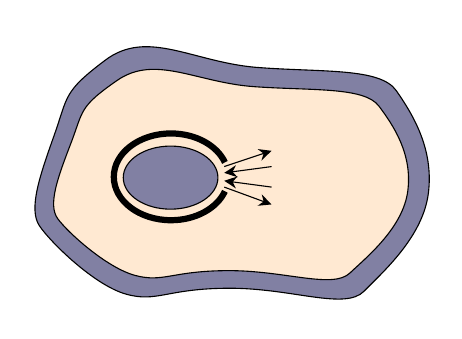
\begin{tikzpicture}[x=0.75pt,y=0.75pt,yscale=-.76,xscale=.76]
				%uncomment if require: \path (0,300); %set diagram left start at 0, and has height of 300
				
				%Shape: Polygon Curved [id:ds9623296108427087] 
				\draw  [color={rgb, 255:red, 0; green, 0; blue, 0 }  ,draw opacity=1 ][fill={rgb, 255:red, 129; green, 128; blue, 163 }  ,fill opacity=1 ] (124.57,48.55) .. controls (151.46,28.29) and (180.41,49.99) .. (221,53.15) .. controls (261.6,56.31) and (298.89,53.15) .. (309.09,67.88) .. controls (319.29,82.62) and (332.79,104.26) .. (329.49,132.34) .. controls (326.19,160.43) and (300.75,182.62) .. (288.69,194.96) .. controls (276.64,207.3) and (243.52,193.09) .. (203.39,193.12) .. controls (163.25,193.15) and (157.53,202.5) .. (137.55,196.8) .. controls (117.57,191.11) and (89.93,164.08) .. (82.84,153.52) .. controls (75.75,142.96) and (83.09,121.82) .. (92.11,96.43) .. controls (101.14,71.04) and (97.68,68.8) .. (124.57,48.55) -- cycle ;
				%Shape: Polygon Curved [id:ds7073560916952666] 
				\draw  [fill={rgb, 255:red, 255; green, 233; blue, 210 }  ,fill opacity=1 ] (131.95,61.48) .. controls (156.15,44.6) and (182.21,62.68) .. (218.75,65.32) .. controls (255.28,67.95) and (288.85,65.32) .. (298.03,77.6) .. controls (307.21,89.87) and (319.36,107.91) .. (316.39,131.31) .. controls (313.42,154.72) and (290.52,173.21) .. (279.67,183.49) .. controls (268.82,193.78) and (239.01,181.94) .. (202.89,181.96) .. controls (166.77,181.98) and (161.62,189.77) .. (143.64,185.03) .. controls (125.65,180.28) and (100.78,157.76) .. (94.4,148.96) .. controls (88.02,140.16) and (94.62,122.55) .. (102.74,101.38) .. controls (110.86,80.22) and (107.75,78.36) .. (131.95,61.48) -- cycle ;
				%Shape: Ellipse [id:dp9298061901489483] 
				\draw  [fill={rgb, 255:red, 129; green, 128; blue, 163 }  ,fill opacity=1 ] (136,123) .. controls (136,111.95) and (149.43,103) .. (166,103) .. controls (182.57,103) and (196,111.95) .. (196,123) .. controls (196,134.05) and (182.57,143) .. (166,143) .. controls (149.43,143) and (136,134.05) .. (136,123) -- cycle ;
				%Shape: Arc [id:dp700197017714294] 
				\draw  [draw opacity=0][line width=2.25]  (200.44,131.66) .. controls (195.47,142.34) and (182.04,150) .. (166.25,150) .. controls (146.23,150) and (130,137.69) .. (130,122.5) .. controls (130,107.31) and (146.23,95) .. (166.25,95) .. controls (182.04,95) and (195.47,102.66) .. (200.44,113.34) -- (166.25,122.5) -- cycle ; \draw  [line width=2.25]  (200.44,131.66) .. controls (195.47,142.34) and (182.04,150) .. (166.25,150) .. controls (146.23,150) and (130,137.69) .. (130,122.5) .. controls (130,107.31) and (146.23,95) .. (166.25,95) .. controls (182.04,95) and (195.47,102.66) .. (200.44,113.34) ;  
				%Straight Lines [id:da7431236595180204] 
				\draw    (200,116) -- (227.15,106.95) ;
				\draw [shift={(230,106)}, rotate = 161.57] [fill={rgb, 255:red, 0; green, 0; blue, 0 }  ][line width=0.08]  [draw opacity=0] (8.04,-3.86) -- (0,0) -- (8.04,3.86) -- (5.34,0) -- cycle    ;
				%Straight Lines [id:da28616458461369365] 
				\draw    (200,129) -- (227.18,138.97) ;
				\draw [shift={(230,140)}, rotate = 200.14] [fill={rgb, 255:red, 0; green, 0; blue, 0 }  ][line width=0.08]  [draw opacity=0] (8.04,-3.86) -- (0,0) -- (8.04,3.86) -- (5.34,0) -- cycle    ;
				%Straight Lines [id:da49527499929740704] 
				\draw    (230,116) -- (202.97,119.6) ;
				\draw [shift={(200,120)}, rotate = 352.41] [fill={rgb, 255:red, 0; green, 0; blue, 0 }  ][line width=0.08]  [draw opacity=0] (8.04,-3.86) -- (0,0) -- (8.04,3.86) -- (5.34,0) -- cycle    ;
				%Straight Lines [id:da8217173823490195] 
				\draw    (230,129) -- (202.97,125.4) ;
				\draw [shift={(200,125)}, rotate = 7.59] [fill={rgb, 255:red, 0; green, 0; blue, 0 }  ][line width=0.08]  [draw opacity=0] (8.04,-3.86) -- (0,0) -- (8.04,3.86) -- (5.34,0) -- cycle    ;
				
				
				
				
			\end{tikzpicture}
			\caption{Esquema del problema.}
			\label{fig:Filtro}
		\end{figure}    
	\end{columns}\pause
	\begin{block}{Principio de equilibrio detallado}
		En equilibrio, la potencia radiada y absorbida por el cuerpo debe ser igual para cualquier elemento de área del cuerpo, dirección de polarización y rango de frecuencias.
	\end{block}
\end{frame}

\begin{frame}{Radiación emitida por un cuerpo}
	\begin{itemize}
		\item Si aplicamos el principio de equilibrio detallado a un cuerpo a temperatura $T$ en equilibrio con la radiación dentro de una caja a esta temperatura.\pause
		\item En una unidad de área del cuerpo tendremos potencia incidente $\mathcal{P}_i(\kv,\alpha)$, de la cual solo una fracción $a(\kv,\alpha)$ es absorbida.\pause
		\item En este proceso una cantidad de potencia $\mathcal{P}_e(-\kv,\alpha)$ es emitida en sentido contrario.
		\item Equilibrando ambos procesos\pause
		\begin{equation}
			\begin{array}{rcl}
				\mathcal{P}_e(-\kv,\alpha) &=& a(\kv,\alpha) \mathcal{P}_i(\kv,\alpha) \\
				\dfrac{\mathcal{P}_e(-\kv,\alpha)}{a(\kv,\alpha)} &=& \mathcal{P}_i(\kv,\alpha)
			\end{array}
			\label{eq:PotBal}
		\end{equation}
		% A la izquierda, solo términos que dependen de la naturaleza del cuerpo y su temperatura.
		% A la derecha, solo términos que dependen de la temperatura dde equilibrio
	\end{itemize}
\end{frame}

\begin{frame}
	\begin{itemize}
		\item A la izquierda de la ecuación \ref{eq:PotBal} solo hay términos dependientes de la naturaleza del cuerpo y su temperatura.
		\item A la derecha, en cambio, solo hay dependencia de la temperatura de equilibrio.\pause
		\item Podemos concluir que la razón del lado izquierdo es dependiente solo de la temperatura.\pause
		% Hay una conexión entre la emisividad y la absorvencia
	\end{itemize}
	\begin{block}{Ley de Kirchhoff}
		\emph{Un buen emisor de radiación es también un buen receptor de emisión, y viceversa}.
		
		Esta conclusión refiere solo a las propiedades del cuerpo, por lo cual es generalmente correcta, incluso si el cuerpo no está en equilibrio.
	\end{block}
\end{frame}

\begin{frame}{Radiación de un cuerpo}
	\begin{itemize}
		\item Un caso particular aparece si consideramos $a(\kv,\alpha) = 1$ para todas las polarizaciones, frecuencias y direcciones de incidencia. Un \emph{cuerpo negro}.\pause
		\item Para este caso, la ecuación \ref{eq:PotBal} se convierte en
		\begin{equation}
			\mathcal{P}_{eb}(-\kv,\alpha) = \mathcal{P}_i(\kv,\alpha)
		\end{equation}
	\end{itemize}
\end{frame}

\begin{frame}
	\begin{columns}
		\column{.65\textwidth}
		\begin{itemize}
			\item Consideremos todos los fotones con vector de onda entre $\kv$ y $\kv+d\kv$.\pause
			% \item Hay $2f(\kv)d^3\kv$ fotones de este tipo (de ambas polarizaciones) por unidad de volumen.
			\item Ya que los fotones se mueven con velocidad $c$ y pueden venir oblicuos al objeto, tendremos que el número promedio de fotones que impactan sobre una unidad de área dependerá del volumen $d^3\kv$ inclinado por un ángulo $\theta$.
			\item Y por lo tanto vendrá dado por $c\hspace{1mm} dt \cos{\theta} f(\kappa) d^3\kv$, con energía $\hbar\omega$ cada uno.\pause
			\item Tendremos que la potencia incidente por unidad de área vendrá dada por
		\end{itemize}
		\begin{equation}
			\begin{array}{rl}
				\mathcal{P}_i(\kv,\alpha)d\omega d\Omega &= \dfrac{d}{dt}(\hbar\omega) (c\hspace{1mm} dt \cos{\theta} f(\kappa) d^3\kv) \\[2ex]
				&= \hbar\omega\ c \cos{\theta} f(\kappa) d^3\kv
			\end{array}
		\end{equation}
		
		\column{.4\textwidth}
		\begin{figure}
			
			
			\tikzset{every picture/.style={line width=0.75pt}} %set default line width to 0.75pt        
			
			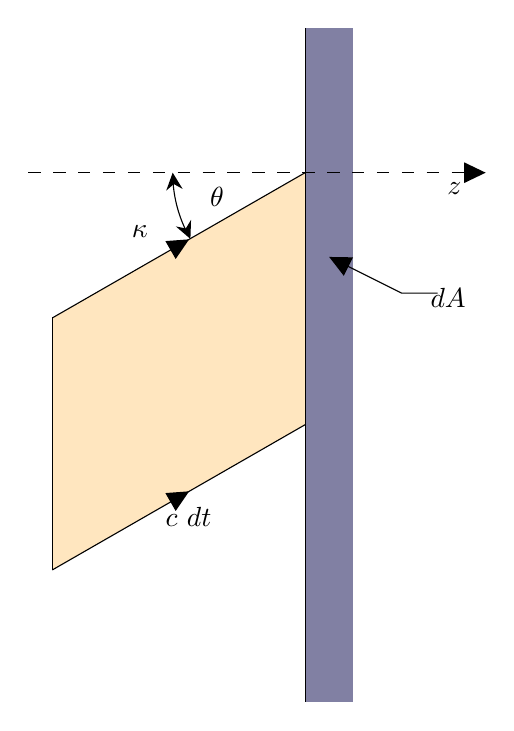
\begin{tikzpicture}[x=.87pt,y=.87pt,yscale=-1,xscale=1]
%				\path (250,450); %set diagram left start at 0, and has height of 300
				
				%Shape: Parallelogram [id:dp1431041402530051] 
				\draw  [draw opacity=0][fill={rgb, 255:red, 255; green, 230; blue, 191 }  ,fill opacity=1 ] (180,174.67) -- (180,70) -- (75,130.33) -- (75,235) -- cycle ;
				%Shape: Rectangle [id:dp17361772387982444] 
				\draw  [draw opacity=0][fill={rgb, 255:red, 129; green, 128; blue, 163 }  ,fill opacity=1 ] (180,10) -- (200,10) -- (200,290) -- (180,290) -- cycle ;
				%Straight Lines [id:da19326483811903972] 
				\draw    (180,10) -- (180,290) ;
				%Straight Lines [id:da6614057187747816] 
				\draw    (75,130.33) -- (180,70) ;
				\draw [shift={(131.84,97.68)}, rotate = 150.12] [fill={rgb, 255:red, 0; green, 0; blue, 0 }  ][line width=0.08]  [draw opacity=0] (8.93,-4.29) -- (0,0) -- (8.93,4.29) -- cycle    ;
				%Straight Lines [id:da1962004417735791] 
				\draw    (75,235) -- (180,174.67) ;
				\draw [shift={(131.84,202.34)}, rotate = 150.12] [fill={rgb, 255:red, 0; green, 0; blue, 0 }  ][line width=0.08]  [draw opacity=0] (8.93,-4.29) -- (0,0) -- (8.93,4.29) -- cycle    ;
				%Straight Lines [id:da01881433151269296] 
				\draw    (75,130) -- (75,235) ;
				%Straight Lines [id:da9652721303942388] 
				\draw  [dash pattern={on 4.5pt off 4.5pt}]  (65,70) -- (252,70) ;
				\draw [shift={(255,70)}, rotate = 180] [fill={rgb, 255:red, 0; green, 0; blue, 0 }  ][line width=0.08]  [draw opacity=0] (8.93,-4.29) -- (0,0) -- (8.93,4.29) -- cycle    ;
				%Straight Lines [id:da4369262336807771] 
				\draw    (235,120) -- (220,120) -- (192.68,106.34) ;
				\draw [shift={(190,105)}, rotate = 26.57] [fill={rgb, 255:red, 0; green, 0; blue, 0 }  ][line width=0.08]  [draw opacity=0] (8.93,-4.29) -- (0,0) -- (8.93,4.29) -- cycle    ;
				%Shape: Arc [id:dp6249591048674698] 
				\draw  [draw opacity=0] (132.36,97.5) .. controls (127.68,89.41) and (125,80.02) .. (125,70) -- (180,70) -- cycle ; \draw    (130.89,94.79) .. controls (127.54,88.16) and (125.49,80.76) .. (125.08,72.92) ; \draw [shift={(125,70)}, rotate = 84.14] [fill={rgb, 255:red, 0; green, 0; blue, 0 }  ][line width=0.08]  [draw opacity=0] (7.14,-3.43) -- (0,0) -- (7.14,3.43) -- (4.74,0) -- cycle    ; \draw [shift={(132.36,97.5)}, rotate = 246.27] [fill={rgb, 255:red, 0; green, 0; blue, 0 }  ][line width=0.08]  [draw opacity=0] (7.14,-3.43) -- (0,0) -- (7.14,3.43) -- (4.74,0) -- cycle    ;
				
				% Text Node
				\draw (107,91) node [anchor=north west][inner sep=0.75pt]   [align=left] {$\displaystyle \kappa $};
				% Text Node
				\draw (121,208) node [anchor=north west][inner sep=0.75pt]   [align=left] {$\displaystyle c\ dt$};
				% Text Node
				\draw (231,117) node [anchor=north west][inner sep=0.75pt]   [align=left] {$\displaystyle dA$};
				% Text Node
				\draw (238,73) node [anchor=north west][inner sep=0.75pt]   [align=left] {$\displaystyle z$};
				% Text Node
				\draw (139.5,75) node [anchor=north west][inner sep=0.75pt]   [align=left] {$\displaystyle \theta $};
				
				
			\end{tikzpicture}
			
		\end{figure}
	\end{columns}
\end{frame}

\begin{frame}
	\begin{itemize}
		\item Expresando el elemento de volumen $d^3\kv$ en coordenadas esféricas, y usando la relación \ref{eq:kappa}, tenemos
		\begin{equation}
			d^3\kv = \kappa^2 d\kappa\hspace{1mm} d\Omega = \dfrac{\omega^2}{c^3}d\omega\hspace{1mm} d\Omega
			\label{eq:KappaEsf}
		\end{equation}\pause
		\item Luego,
		\begin{equation}
			\mathcal{P}_i(\kv,\alpha) = \dfrac{\hbar\omega^3}{c^2}f(\kappa) \cos{\theta} 
		\end{equation}\pause
		\item Este resultado no depende de la dirección de polarización $\alpha$, pero sí del ángulo de incidencia respecto a la normal a la superficie $\theta$.
	\end{itemize}
\end{frame}

\begin{frame}
	\begin{itemize}
		\item Considerando el balanceo de la ec. \ref{eq:PotBal}
		\begin{equation}
			\mathcal{P}_e(\kv',\alpha)\hspace{1mm}d\omega\hspace{1mm}d\Omega = a(-\kv',\alpha)\hspace{1mm}\dfrac{\hbar\omega^3}{c^2}f(\kappa) \cos{\theta}\hspace{1mm}d\omega\hspace{1mm}d\Omega
			\label{eq:PotExp}
		\end{equation}\pause
		\item Si el cuerpo absorbe isotrópicamente, tal que $a(-\kv',\alpha)$ es independiente de la dirección $\kv'$, se demuestra que la potencia emitida es proporcional al $\cos{\theta}$. Este resultado es conocido como la \emph{Ley de Lambert}.
	\end{itemize}
\end{frame}

\begin{frame}
	\begin{itemize}
		\item Encontremos ahora la potencia total $\mathcal{P}_e(\omega)d\omega$ emitida por unidad de área en el intervalo de frecuencias $\omega$ y $\omega+d\omega$ para ambas direcciones de polarización.\pause
		\item Integrando la ec. \ref{eq:PotExp} sobre todas las direcciones de emisión, multiplicando por 2 para considerar ambas direcciones de polarización, asumiendo $a = a(\omega)$ independiente de la dirección y polarización, y tomando $d\Omega = \sin{\theta} \hspace{1mm} d\theta \hspace{1mm} d\phi$\pause
		\begin{equation}
			\begin{array}{rcl}
				\mathcal{P}_e(\omega)d\omega &=& 2\int_\Omega \mathcal{P}_e(\kv',\alpha) d\omega\hspace{1mm}d\Omega \\[1ex]
				&=& a(\omega)\dfrac{2\hbar\omega^3}{c^2}f(\kappa)d\omega\left(2\pi\displaystyle\int_0^{\pi/2}\cos{\theta}\sin{\theta}d\theta\right) \\[1ex]\pause
				\mathcal{P}_e(\omega)d\omega &=& a(\omega)\dfrac{2\pi\hbar\omega^3}{c^2}f(\kappa)d\omega
			\end{array}
			\label{eq:PotTot}
		\end{equation}
	\end{itemize}
\end{frame}

\begin{frame}
	\begin{itemize}
		\item Podemos utilizar el resultado de la ec. \ref{eq:DensEnerProm} para escribir la expresión \ref{eq:PotTot} como
		\begin{equation}
			\mathcal{P}_e(\omega)d\omega = a(\omega)\left(\frac{1}{4}c\bar{u}(\omega)\hspace{1mm}d\omega\right)
		\end{equation}\pause
		\item O la expresión \ref{eq:DensFot} para $f(\kappa)$, con la ec. \ref{eq:KappaEsf} para $d\kappa^3$, para obtener
		\begin{equation}
			\mathcal{P}_e(\omega)d\omega = a(\omega)\frac{\hbar}{4\pi^2c^2}\frac{\omega^3d\omega}{e^{\beta\hbar\omega}-1}
		\end{equation}
	\end{itemize}
\end{frame}

\begin{frame}{Radiación de un cuerpo negro}
	\begin{itemize}
		\item Si tenemos que $a(\omega) = 1$, es decir, un cuerpo que absorbe toda la luz de todas las frecuencias, tendremos para la expresión anterior
		\begin{equation}
			\mathcal{P}_{eb}(\omega)d\omega = \frac{\hbar}{4\pi^2c^2}\frac{\omega^3d\omega}{e^{\beta\hbar\omega}-1}
		\end{equation}
		también conocida como \emph{Ley de Planck para la distribución espectral de radiación de cuerpo negro}.
	\end{itemize}
\end{frame}

\begin{frame}
	\begin{figure}
		\centering
		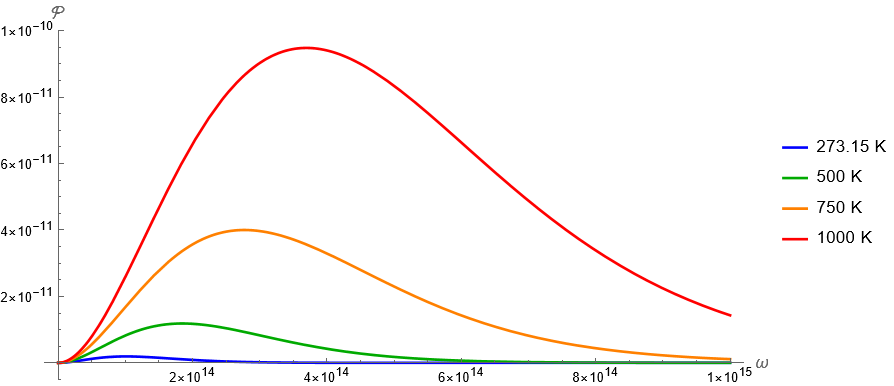
\includegraphics[width=\textwidth]{images/espectro}\caption{Espectro de emisión sobre frecuencia angular para 4 cuerpos negros a distinta temperatura.}
		\label{fig:Espectro}
	\end{figure}    
\end{frame}

\begin{frame}
	\begin{itemize}
		\item Finalmente, podemos integrar sobre todas las frecuencias para obtener la potencia \emph{total} $\mathcal{P}_e^{(0)}$ emitida por unidad de área.\pause
		\item Si $a(\omega)$ tiene un valor constante $a$ en los rangos de frecuencias para los que $\mathcal{P}_e$ no es despreciable, tendremos la llamada \emph{Ley de Stefan-Boltzmann}
		\begin{equation}
			\mathcal{P}_e^{(0)} = a\left(\frac{1}{4}c\bar{u}\right) = a(\sigma T^4)
		\end{equation}
		donde $\sigma$ corresponde a la constante de Stefan-Boltzmann \[\sigma\equiv\dfrac{\pi^2}{60}\dfrac{k_B^4}{c^2\hbar^3} = (5.6697\pm0.0029)\times 10^{-5} \text{erg sec}^{-1}\text{ cm}^{-2}\text{ deg}^{-4}\]
	\end{itemize}
\end{frame}
%%%%%%%%%%%%%%%%%%%%%%%%%%%%%%%%%%%%%%%%%%%%%%%%%%%%%%%%



















\end{document}